\documentclass[20pt,a4paper,landscape]{extarticle}
\usepackage[margin=1.25in]{geometry}
\usepackage{placeins}
\usepackage{latexsym}
\usepackage{marvosym}
\usepackage[utf8]{inputenc}
\usepackage[T1]{fontenc}
\usepackage[UKenglish]{babel}
\usepackage[UKenglish]{isodate}
\usepackage{amsmath}
\usepackage{amsfonts}
\usepackage{amssymb}
\usepackage{amsthm}
\usepackage{graphicx}
\usepackage{titletoc}
\PassOptionsToPackage{hyphens}{url}
\usepackage{xurl}
\input{glyphtounicode}
\pdfgentounicode=1
\usepackage[all]{nowidow}
\usepackage{hyperref}
\hypersetup{
    colorlinks,
    citecolor=black,
    filecolor=black,
    linkcolor=black,
    urlcolor=black
}
\usepackage[protrusion=true,expansion=true]{microtype}
\newcommand{\ind}{\perp\!\!\!\!\perp}
\begin{document}
\tableofcontents
\clearpage
\begin{flushleft}
\section{The Lambda Calculus}
\subsection{Foundations}
\begin{itemize}
\item \textbf{Application} is left-associative and \textbf{binds more tightly than abstraction}: $\lambda x. M_1M_2M_3 \equiv \lambda x. (M_1M_2M_3) \equiv \lambda x. (M_1M_2)M_3$
    \begin{itemize}
    \item Thus, abstraction is right associative
    \end{itemize}
\item \textbf{De-Bruijn notation} is a compact way of expressing $\lambda$-calculus expressions: Each instance of a lambda (together with the variable it binds) creates a \verb|[| and each use of a variable is replaced by a number showing how many \verb|[| there are to the left of it up to and including the one that bound it \textbf{e.g. $\lambda x. x(\lambda y. y (x x))$ becomes [1[1 (2 2)]]}
\clearpage
\item \textbf{Capture avoidance: Free variables cannot become bound, other than if they have been abstracted away} — scope
\item \textbf{Freshness: Variables that have been bound cannot be reused} — immutability
\item FV($M$) = set of free variables in the term $M$
\item \textbf{$\alpha$-reduction: $\lambda x. M \underset{\alpha}{\rightarrow} \lambda y. M[x \leftarrowtail y]$ if $y \notin \textrm{FV}(M)$} — find and replace all
\item $\alpha$-equivalence: Expressions are $\alpha$-equivalent iff one can be obtained from the other by a series of $\alpha$-reductions
\end{itemize}
\clearpage
\subsection{Contractions}
\begin{itemize}
\item \textbf{$\beta$-reduction (contraction): $(\lambda x. M)N \underset{(\beta)}{\rightarrow} M[x \leftarrowtail N]$} — function application
    \begin{itemize}
    \item The abstraction which the application is happening to is called the redex
    \item A series of $\beta$-reductions is called a reduction sequence — this is the process by which actual computation will happen
    \end{itemize}
\item \textbf{$\eta$-reduction (eta-reduction): $\lambda x. Mx \underset{\eta}{\rightarrow} M$} — if all an abstraction does is function application, we can discard it as we already have function application as an implicit part of our language
    \begin{itemize}
    \item Arises from $\beta$-reduction: $(\lambda x. Mx)N \rightarrow MN$
    \end{itemize}
\end{itemize}
\subsection{Evaluation}
\begin{itemize}
\item $A \Rightarrow B$ ($A$ evaluates to $B$) iff there exists a reduction sequence that takes $A$ to $B$ \underline{and B is a normal form}
    \begin{itemize}
    \item \underline{There may be multiple reduction sequences from a given term, only}\\
    \underline{some of which may converge}
    \item Normal forms are unique: All convergent reduction sequences from one term converge upon the same normal form
    \end{itemize}
\item $\nexists B: A \Rightarrow B$ iff $A$ diverges (throws an error or causes an infinite loop)
\item \textbf{Normal reduction order = always reduce the leftmost redex}
\item \textbf{Applicative reduction order = always reduce the rightmost redex}
\item Normal order is guaranteed to find a normal form if one exists (whereas applicative is not)
\end{itemize}
\subsection{Normal forms}
\begin{itemize}
\item Let $E, E_1, ..., E_n$ be expressions in the relevant normal form
\item Let $e, e_1, ..., e_n$ be expressions (may or may not be in the normal form)
\item \textbf{(Full) Normal form} (NF) = $\lambda x. E$ | $xE_1...E_n$ | $x$
    \begin{itemize}
    \item There really is no way to simplify it: \textbf{Cannot be $\beta$-reduced}
    \end{itemize}
\item \textbf{Head normal form} (HNF) = $\lambda x. E$ | $xe_1...e_n$ | $x$
    \begin{itemize}
    \item \textbf{Arguments of applications are not required to be $\beta$-irreducible but bodies of abstractions are}
    \item \textit{The lazy normal form of theoreticians}
    \end{itemize}
\clearpage
\item \textbf{Weak head normal form} (WHNF) = $\lambda x. e$ | $xe_1...e_n$ | $x$
    \begin{itemize}
    \item \textbf{Outermost term is not an application where the LHS is an abstraction}
    \item \textit{The lazy normal form of actual programming languages}
    \end{itemize}
\item \textbf{Weak normal form} (WNF) = $\lambda x. e$ | $xE_1...E_n$ | $x$
    \begin{itemize}
    \item \textbf{No applications anywhere that could be evaluated unless they are within an abstraction}
    \item \textit{Seemingly only included for completeness}
    \end{itemize}
\item If in NF, then in HNF and in WNF
\item If in HNF, then in WHNF
\item If in WNF, then in WHNF
\end{itemize}
\subsection{Combinators}
\begin{itemize}
\item Combinators abbreviate commonly used \underline{closed} (no free variables) $\lambda$-calculus expressions
\item The definitions of any specific combinators needed will be included in the exam
\item Any closed form $\lambda$-calculus expression can be written using only the S ($\lambda x.y.z. x z (y z)$)  and K ($\lambda x.y. x$) combinators
    \begin{itemize}
        \item \textit{As the $\lambda$-calculus is Turing complete and an expression can be fully evaluated only if it is closed, any computable function can be written only using the S and K combinators}
    \end{itemize}
\end{itemize}
\clearpage
\section{Explicit Typing (STLC and PCF)}
\subsection{Terminology for proof rules}
\begin{itemize}
\item An environment = an association of values to free variables
    \begin{itemize}
        \item Type environment = list of pairs of \underline{variables} and their types
    \end{itemize}
\item A judgment = an evaluation of an expression given an environment
    \begin{itemize}
        \item Typing judgment = evaluation of the type of a \underline{term} in a given type environment
    \end{itemize}
\item A derivation = a proof of a judgement using steps of axiomatic smaller judgements
\end{itemize}
\subsection{Syntax of the simply typed lambda calculus (STLC)}
\begin{itemize}
\item Simply typed means the only base type is a generic value (o) and all other types are functions on types
\item The syntax of the STLC has explicit type annotations on the lambda bindings of variables (and only here)
\end{itemize}
\clearpage
\subsection{Typed evaluation rules (dynamic semantics) for STLC}
\FloatBarrier
\begin{figure}[h]
\begin{center}
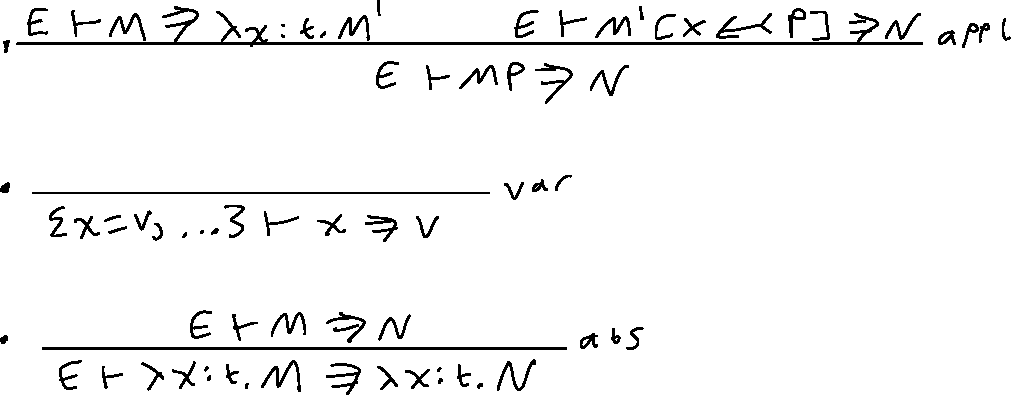
\includegraphics[width=\textwidth]{meta/cs349/STLC_Rules_Eval.pdf}{}
\end{center}
\end{figure}
\FloatBarrier
\clearpage
\subsection{Typing rules (static semantics) for STLC}
\FloatBarrier
\begin{figure}[h]
\begin{center}
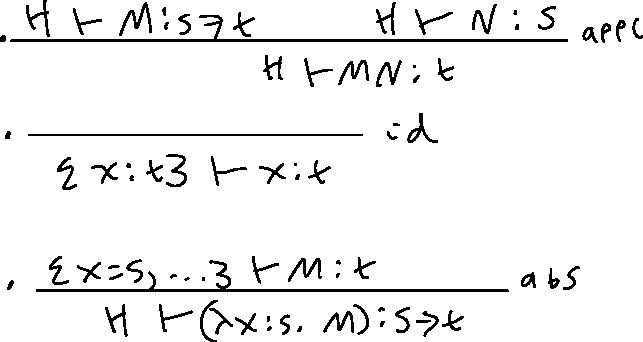
\includegraphics[width=0.81\textwidth]{meta/cs349/STLC_Rules_Typing.pdf}{}
\end{center}
\end{figure}
\FloatBarrier
Subject reduction theorem: Reduction to a normal form preserves the type of an expression
\clearpage
An example of static semantics:
\begin{figure}[h]
\begin{center}
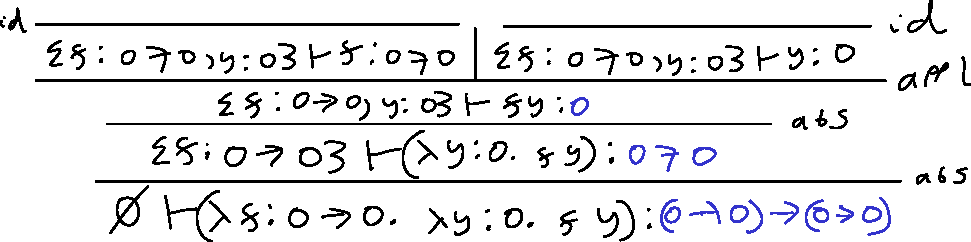
\includegraphics[width=\textwidth]{meta/cs349/STLC_Rules_Example.pdf}{}
\end{center}
\end{figure}
\FloatBarrier
Proof trees are built bottom to top but verified (and types are filled in) top-to-bottom
\clearpage
\subsection{PCF (Programming with Computable Functions)}
\begin{itemize}
\item PCF extends the STLC by introducing distinct base types for different classes of value and allowing let-declarations (of constants \underline{not variables})
\begin{itemize}
    \item \textit{As $\lambda$-calculus (even the S and K combinators alone) was Turing-complete, PCF is not literally more powerful but it is far more convenient to have syntactic sugar than to have to encode numerals in unary with function compositions etc. Also, a more expressive type system allows stronger correctness guarantees}
\end{itemize}
\item Base types are num (n) and bool (b) --- num refers to Church numerals (naturals (hence the operations we define for them)) not a more general class of numbers
\item $t$ := n | b | $t \ast t$ | $t \mapsto t$
\item $M$ := 0 | 1 | 2 | ... | true | false | succ$(M)$ | pred$(M)$ | zero?$(M)$ | $M + M$ | $M \times M$ | $\langle M, M \rangle$ | fst$(M)$ | snd$(M)$ | if $M$ then $M$ else $M$ | $x$ | $\lambda x: t. M$ | $M M$ | let $d$ in $M$\\
$d$ := ($x = M$) | $d$ and $d$
\end{itemize}
\clearpage
\subsection{PCF Dynamic Semantics}
\begin{figure}[h]
\begin{center}
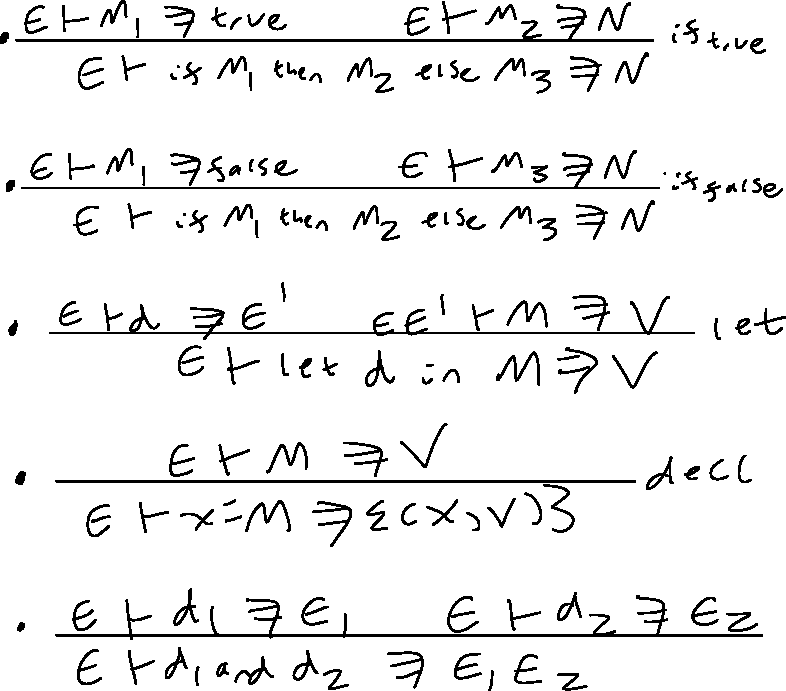
\includegraphics[width=0.5\textwidth]{meta/cs349/PCF_Eval.pdf}{}
\end{center}
\end{figure}
\FloatBarrier
\begin{itemize}
\item Note that \textbf{declarations ``evaluate'' into additional environments} rather than expressions
\item \textbf{Applications are evaluated using lazy evaluation} (substitute then evaluate whole expression) \textbf{whereas declarations use eager evaluation} (evaluate before substituting (then do the new remaining evaluation))
\item When two environments are placed next to each other (e.g. $EE'$) they are implicitly unioned and this is done in a way that respects the scope of bindings (e.g. let $x=1$ in let $x=2$ in $x$ $\Rightarrow$ 2)
\end{itemize}
\clearpage
\subsection{PCF Static Semantics}
\begin{figure}[h]
\begin{center}
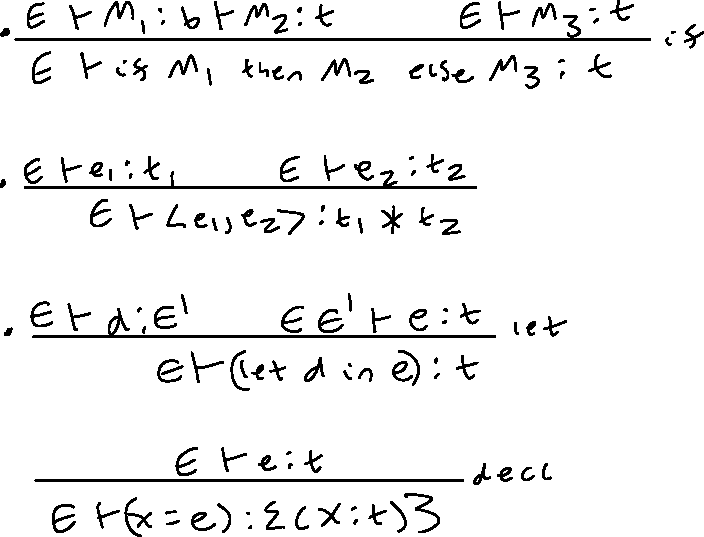
\includegraphics[width=0.57\textwidth]{meta/cs349/PCF_Typing.pdf}{}
\end{center}
\end{figure}
\FloatBarrier
Note that each branch of an if must be assigned the same type

An example:
\FloatBarrier
\begin{figure}[h]
\begin{center}
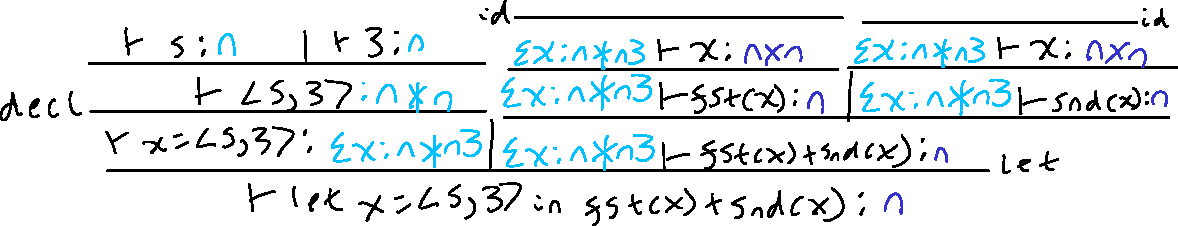
\includegraphics[width=\textwidth]{meta/cs349/PCF_Typing_Example.pdf}{}
\end{center}
\end{figure}
\FloatBarrier
Note that the rules for \verb|+|, \verb|fst| etc are common sense
\clearpage
\section{Miscellaneous Content}
\subsection{Recursion}
\begin{itemize}
\item A function in the $\lambda$-calculus cannot directly refer to itself in its own definition, but the $Y$ combinator applies a function infinitely many times\textbf{: $Yf \rightarrow f(Yf) \rightarrow f(f(Yf)) \rightarrow ...$}
\item $Y = \lambda f. (\lambda x. f(xx))(\lambda x. f(xx))$
\item Under strict evaluation the Y-combinator is useless as everything diverges under it, but under lazy evaluation recursive functions are evaluated down to their base case then return
\item \textbf{$Y(\lambda f. M)$ is abbreviated to $\mu f. M$}
\FloatBarrier
\begin{figure}[h]
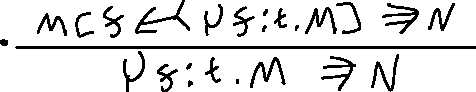
\includegraphics[width=0.5\textwidth]{meta/cs349/YComb_Natural.pdf}{}
\end{figure}
\FloatBarrier
\item \textit{The dynamic semantics of functions on numbers are recursive (Peano arithmetic) --- the fact the halting problem exists by sometimes divergent terms such as the $Y$ combinator is the price we pay for expressiveness}
\end{itemize}
\subsection{Structural Semantics}
\begin{itemize}
\item So far we have mainly considered natural semantics ($\Rightarrow$), how an expression becomes a normal form.
\item Structural semantics ($\rightarrow$) describe the step-by-step process of evaluation
\item By convention we evaluate left-to-right
\clearpage
\item Call-by-name is lazy (as have been our natural semantics):
\FloatBarrier
\begin{figure}[h]
\begin{center}
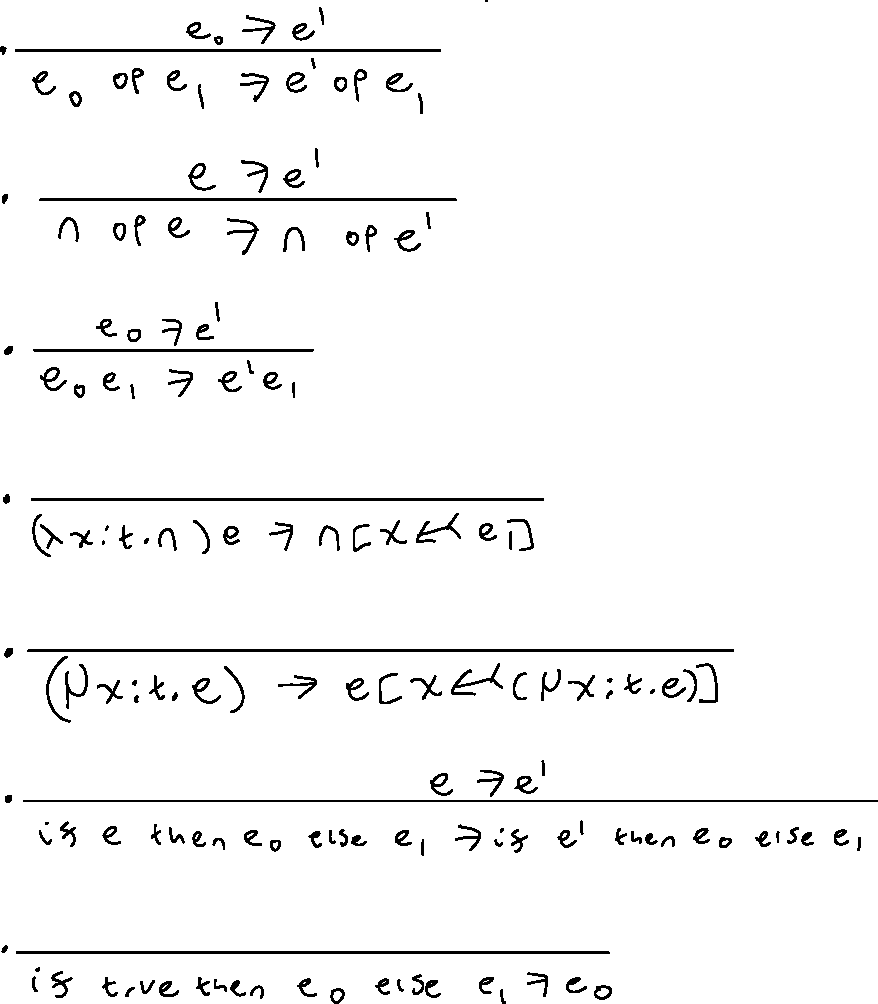
\includegraphics[width=0.38\textwidth]{meta/cs349/CBN_Structural.pdf}{}
\end{center}
\end{figure}
\clearpage
\item Call-by-value is eager, only requires some changes to call-by-name:
\FloatBarrier
\begin{figure}[h]
\begin{center}
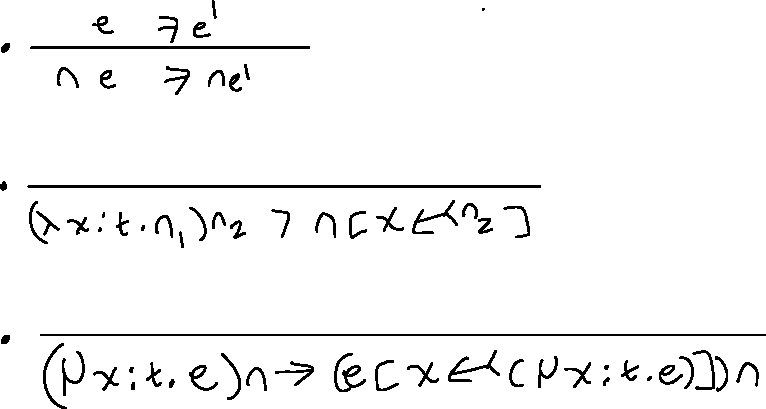
\includegraphics[width=0.82\textwidth]{meta/cs349/CBV_Structural.pdf}{}
\end{center}
\end{figure}
\FloatBarrier
\end{itemize}
\clearpage
\subsection{Type theory}
\begin{itemize}
\item \textbf{Curry-Howard Isomorphism: Types are propositions and vice versa. Moreover, the type of every closed expression is a tautology.}
    \begin{itemize}
    \item $\mapsto$ is isomorphic to logical implication (including being right associative like it), $\ast$ is isomorphic to logical conjunction etc
    \item \textit{Functions can curried because $(A \land B) \rightarrow C \equiv A \rightarrow (B \rightarrow C)$}
    \end{itemize}
\end{itemize}
\clearpage
\subsection{Type judgements}
\begin{itemize}
\item Types allowed us to check that terms were well-formed but Cardelli's type judgements will allow us to check that types themselves are well-formed
\textbf{
\item $\Gamma \vdash \diamond$ means the environment $\Gamma$ is well formed
\item $\Gamma \vdash T$ means the the type $T$ is well formed in $\Gamma$
\item $\Gamma \vdash M : T$ means the the term $M$ has type $T$ (and so is well formed) in $\Gamma$
}
\end{itemize}
\FloatBarrier
\begin{figure}[h]
\textbf{Cardelli rules:}
\begin{center}
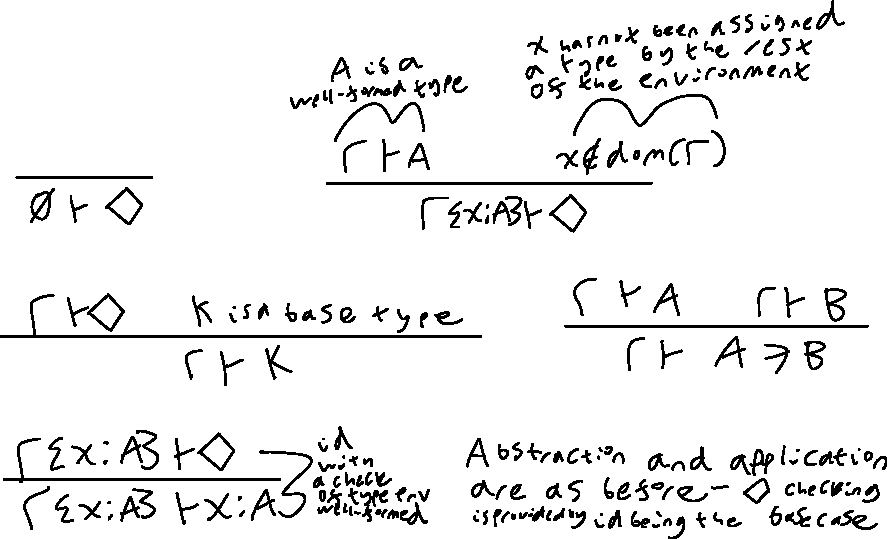
\includegraphics[width=0.72\textwidth]{meta/cs349/Cardelli.pdf}{}
\end{center}
Additional rules for well-formed types will arise as our type system becomes richer (e.g. polymorphic types) but these follow the same pattern as the function type rule shown above.
\end{figure}
\FloatBarrier
\FloatBarrier
\begin{figure}[h]
Type trees begin much as before but now continue past the id term rule to only bottom out at empty environment is well formed. An example:
\begin{center}
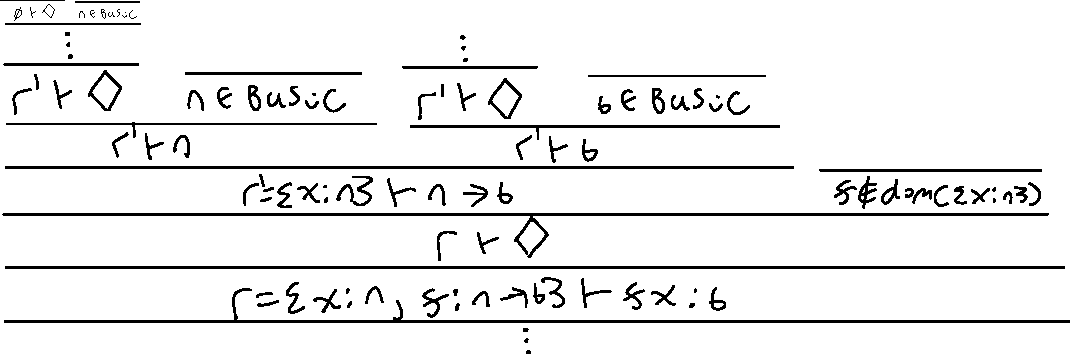
\includegraphics[width=\textwidth]{meta/cs349/Cardelli_Example.pdf}{}
\end{center}
Note that at \underline{each check of the environment admitting a type, that type is}\\
\underline{removed from the environment}
\end{figure}
\FloatBarrier
\clearpage
\section{Implicit Typing (MiniML)}
\subsection{MiniML}
\begin{itemize}
\item MiniML uses \verb|fn| instead of $\lambda$ but otherwise the only notable difference to PCF is the use of type inference instead of explicit typing. (If we carried on using $\lambda$, then MiniML expressions could be confused for untyped lambda calculus expressions)
\end{itemize}
\subsection{Polymorphism}
\begin{itemize}
\item MiniML (sort of) has universally quantified types, which allows it to have lists
    \begin{itemize}
    \item \verb|nil|: $\forall \alpha. \alpha$ \verb|list|
    \item \verb|::|: $\forall \alpha. \alpha \ast \alpha$ \verb|list| $\mapsto \alpha$ \verb|list|
    \item \verb|hd|: $\forall \alpha. \alpha$ \verb|list| $\mapsto \alpha$
    \end{itemize}
\item $\forall$s are not actually allowed in MiniML types, instead MiniML has so called type schemes which do allow $\forall$
\item Type schemes allow sub-terms to be universally quantified as an intermediate step in deriving a true type for a fully formed term (the context will cause the type scheme to specialise into a particular type)
\item Closure of the type scheme of a type expression $\sigma$ in a typing environment T = $\textrm{CL}_\textrm{T}(\sigma) = \forall \alpha_1...\alpha_n.\sigma$ where $\alpha_1...\alpha_n$ are the free variables in $\sigma$ (do not occur in T)
\item As well as there being polymorphic built-ins (lists), programmers can create polymorphic functions of a sort. This is achieved by using a let ... in ... to declare the generic function then immediately use it in a particular context
\clearpage
\item \textbf{The type environment produced by a declaration is (in generality) the closed type scheme arising from the type expression of the definition}, we just didn't realise before because previously we had no free variables so it was implicitly closed
\end{itemize}
\subsection{Type inference}
Hindley-Damas-Milner type inference algorithm:
\textbf{
\begin{enumerate}
\item Build tree of type variables using structural induction over terms --- create a fresh type variable for each instance of a universal quantifier
\item Build a set of constraints based on the rules used to build the tree (using $\sim$ to denote an equivalence relation on types). A constraint that a closure $C_i$ instantiates into a type variable $t_j$ of a particular form is written as $C_i \succ t_j \sim ...$
\item Combine constraints to find the most general unifier at each level and so eventually at the root --- consume by substituting into each other until only the type at the root remains. Even if the type of the root is found early, all constraints must be consumed to check that nothing has been assigned an additional incompatible type
\end{enumerate}
}
\begin{itemize}
\item \textit{PCF has roughly the most powerful type system for which type checking (and so certainly type inference) is not in general undecidable}
\end{itemize}
\clearpage
\textbf{
Constraints:
\FloatBarrier
\begin{figure}[h]
\begin{center}
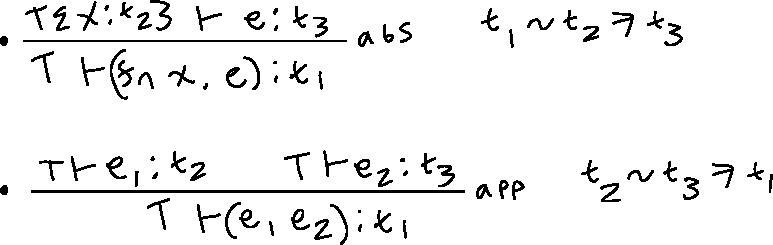
\includegraphics[width=\textwidth]{meta/cs349/UnificationRules.pdf}{}
\end{center}
\end{figure}
}
\begin{itemize}
\item Note that the application rule is written in terms of abstraction
\end{itemize}
\clearpage
Types unify if (this makes it sound complicated but is it actually very intuitive):
\begin{itemize}
\item They are the same base type (e.g. both are int)
\item One is a type variable and the other is not a type expression in which that type variable occurs
\item They are the same type constructor and the sub expressions unify (e.g. are list $\tau_1$ and list $\tau_2$ and $\tau_1 \sim \tau_2$)
\end{itemize}
If types cannot be unified, the expression is illegal so a type error is raised
\clearpage
Example of legal expression:
\FloatBarrier
\begin{figure}[h]
\begin{center}
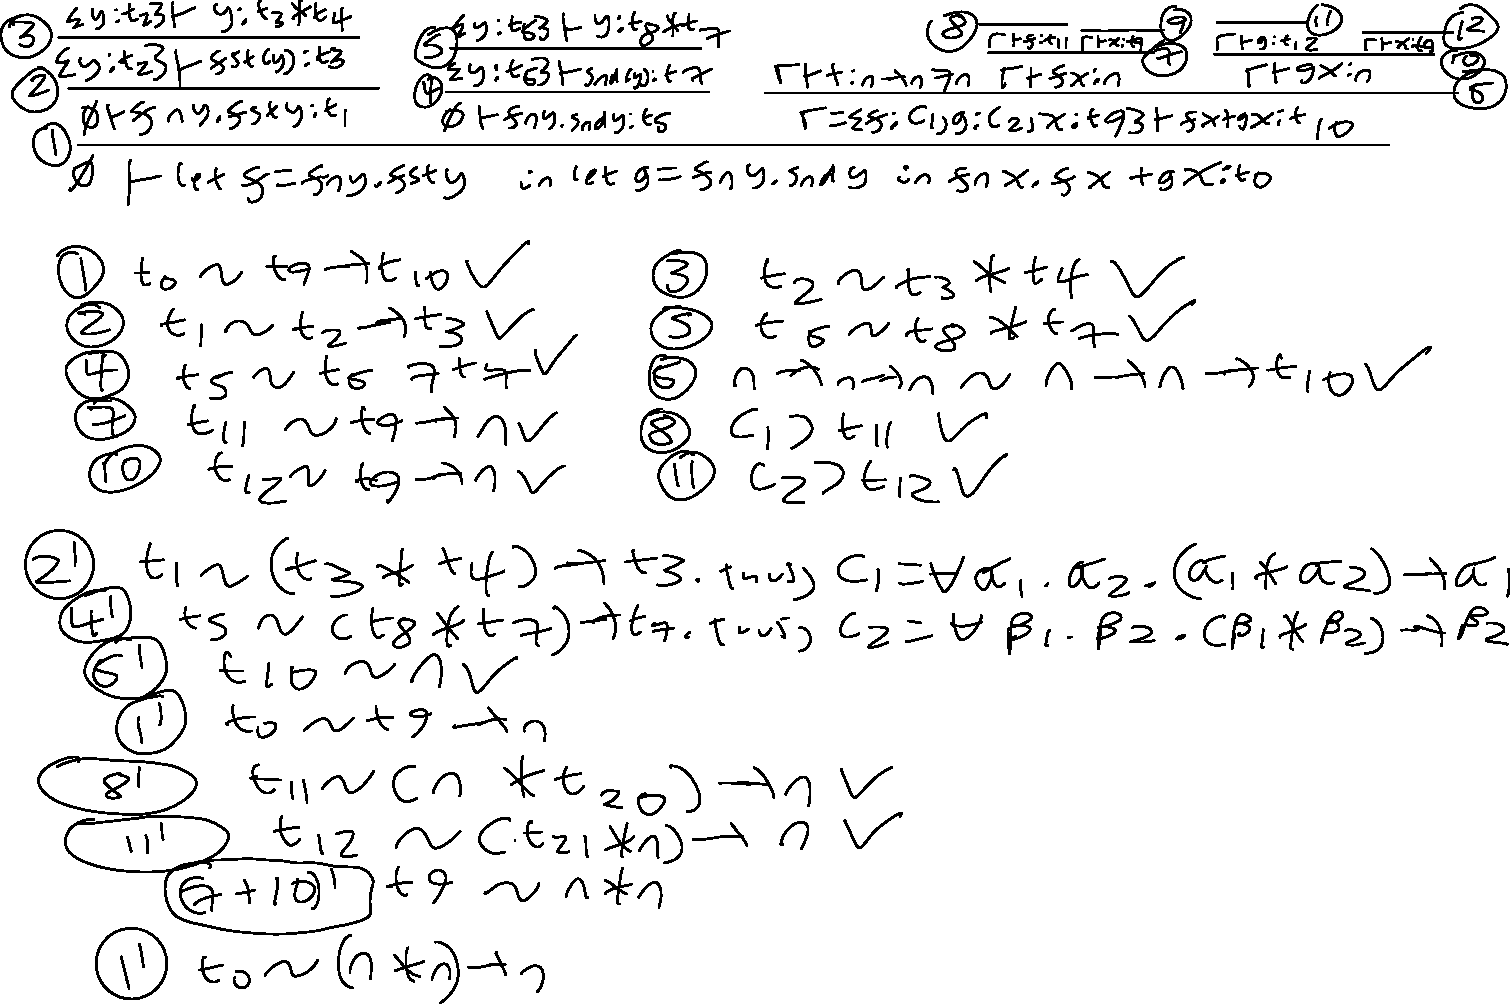
\includegraphics[width=0.66\textwidth]{meta/cs349/HTMI_Example4.pdf}{}
\end{center}
\end{figure}
\clearpage
Example of un-typeable expression:
\begin{figure}[h]
\begin{center}
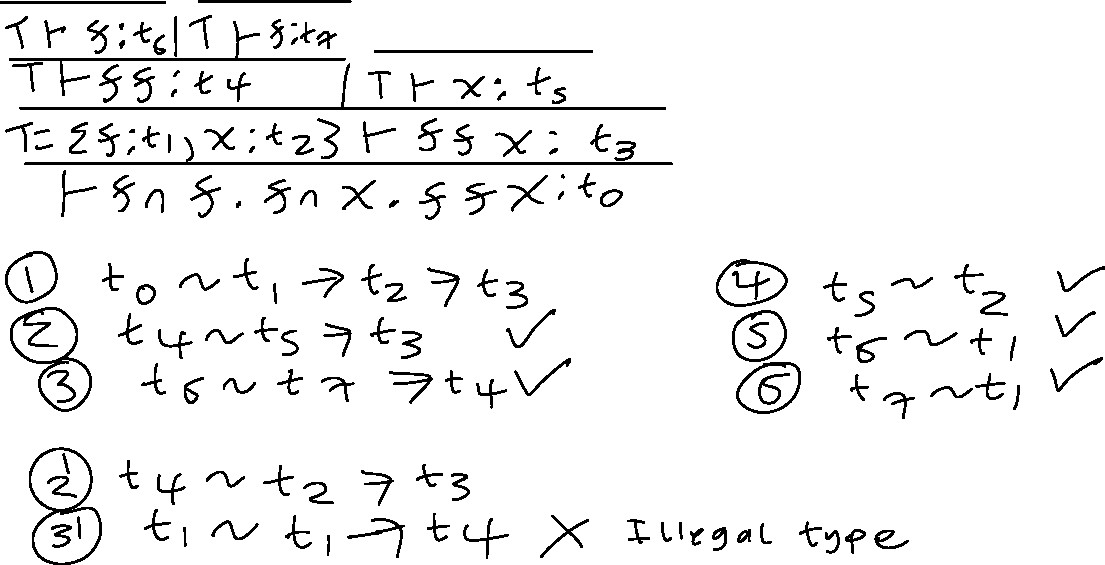
\includegraphics[width=0.86\textwidth]{meta/cs349/HTMI_Example2.pdf}{}
\end{center}
\end{figure}
\FloatBarrier
\textit{This expression is actually well-formed but can only be assigned a recursive type (which this system isn't powerful enough to do)}\\
However we have enough polymorphism to be able to handle this if we already know the general definition of f:
\FloatBarrier
\begin{figure}[h]
\begin{center}
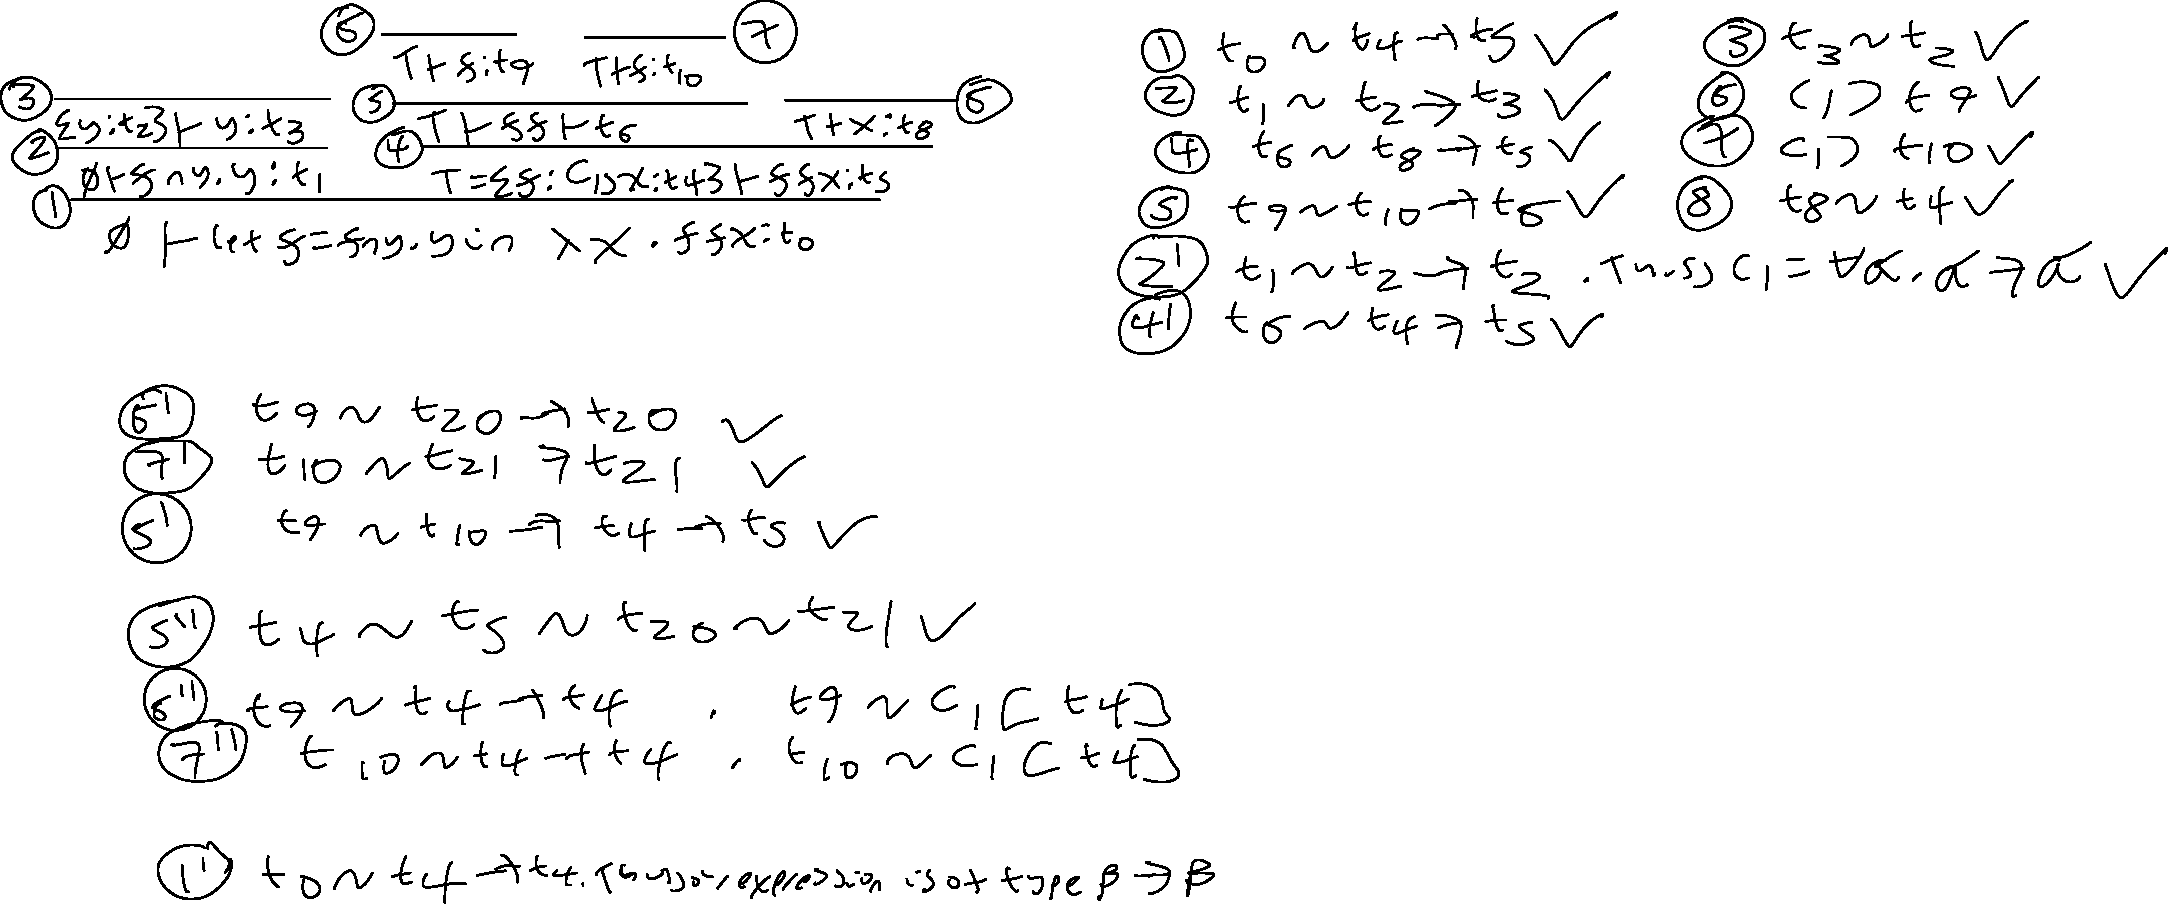
\includegraphics[width=0.99\textwidth]{meta/cs349/HTMI_Example3.pdf}{}
\end{center}
\end{figure}
\FloatBarrier
Note that each invocation of a polymorphic function can instantiate it with fresh type variables
\section{Quantified Types (PLC and SLS)}
\subsection{PLC}
\begin{itemize}
\item Although MiniML implicitly had polymorphism, polymorphic $\lambda$-calculus (PLC) has polymorphic types as a part of the language itself, however this means that we revert to explicit typing
    \begin{itemize}
    \item \textit{As type checking now requires checking for a tautology in first-order logic instead of propositional logic, it is now undecidable}
    \end{itemize}
\item \textbf{A capital lambda ($\Lambda$) denotes a type-level function as opposed to a value-level function ($\lambda$)} --- these generic expressions genuinely have a universally quantified type
\item \underline{A generic expression $e$ must be instantiated with a particular type}\\\underline{expression $t$ ($e[t]$) before it can be used}
\end{itemize}
\FloatBarrier
\begin{figure}[h]
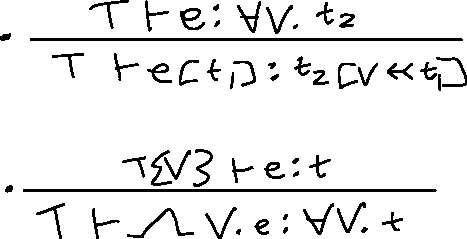
\includegraphics[width=0.45\textwidth]{meta/cs349/PLC_TypingRules.pdf}{}
\end{figure}
\FloatBarrier
Note that the first rule resembles the one for (value-level) application and the second rule resembles the one for (value-level) abstraction. Note that we are now allowing lone type variables to be members of our type environments.

Example: bool = $\forall \alpha. \alpha \mapsto (\alpha \mapsto \alpha)$ and False = $\Lambda \alpha. \lambda x_1: \alpha. \lambda x_2: \alpha. x_2$. Show that False: bool.
\FloatBarrier
\begin{figure}[h]
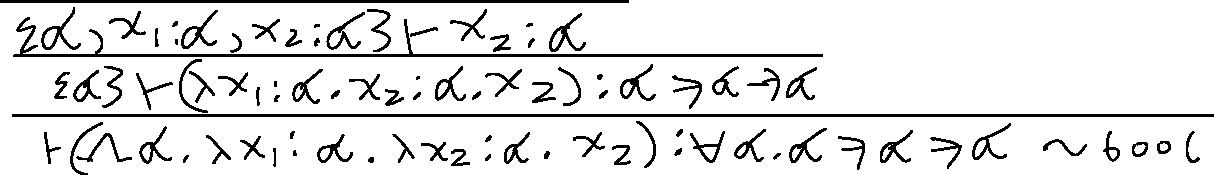
\includegraphics[width=\textwidth]{meta/cs349/PLC_Example.pdf}{}
\end{figure}
\FloatBarrier
\subsection{Subtyping}
\begin{itemize}
\item $S<:T$ = $S$ is a subtype of $T$
    \begin{itemize}
    \item \underline{This is actually reflexive} but this is the standard notation
    \end{itemize}
\item $T$ occurs co-variantly in $F[T]$ iff ($F[T_1]$ $<:$ $F[T_2]$ iff $T_1$ $<:$ $T_2$) \textit{--- producers (i.e. writing data i.e. function return values) can produce more than is needed}
\item $T$ occurs contra-variantly in $F[T]$ iff ($F[T_1]$ $<:$ $F[T_2]$ iff $T_1$ $>:$ $T_2$) \textit{--- consumers (i.e. reading data i.e. function parameters) can consume less than they are given}
\item $T$ occurs in-variantly in $F[T]$ iff ($F[T_1]$ $<:$ $F[T_2]$ iff $T_1$ = $T_2$) \textit{--- mutable data can be written and read so must be co- and contra-variant so as the types must obey the ordering relation in both directions they must be equal}
\item \textit{PECS: Producer Extends, Consumer Super}
\end{itemize}
\FloatBarrier
\begin{figure}[h]
\begin{center}
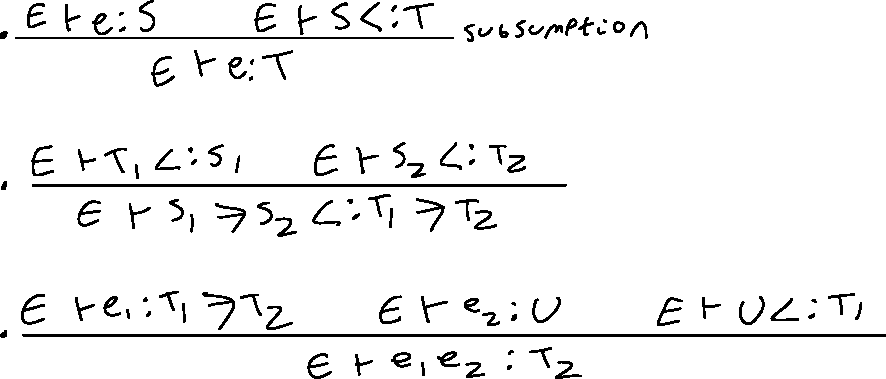
\includegraphics[width=0.86\textwidth]{meta/cs349/Subtype_Rules.pdf}{}
\end{center}
\end{figure}
\FloatBarrier
\begin{itemize}
\item The first rule encodes the Liskov substitution principle (behavioural sub-typing): If S is a subtype of T, then an expression of type T may be replaced with an expression of type S without altering the semantic properties of the program
\item The second rule encodes the fact that function arguments are contravariant and function return values are covariant
\item The third rule is a corollary of the first two but corresponds to the fact that it is advisable to consider sub-typing lazily (most rules are guaranteed to make progress as they break down the syntax of terms whereas subsumption can in principle be applied infinitely many times)
\end{itemize}
\subsection{Records}
\begin{itemize}
\item A record associates expressions with labelled fields
\item A particular field of a record is accessed using @
\FloatBarrier
\begin{figure}[h]
\begin{center}
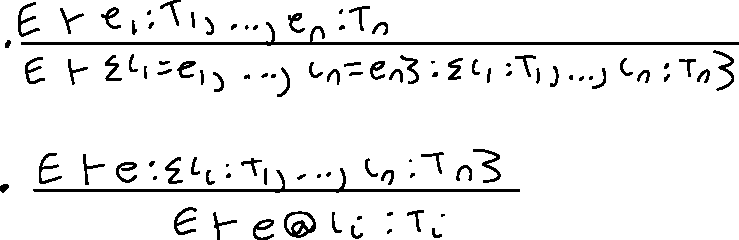
\includegraphics[width=0.86\textwidth]{meta/cs349/Records_Rules.pdf}{}
\end{center}
\end{figure}
\FloatBarrier
\item Note that the type of a record is itself a record of sorts
\item \textbf{A record is a \underline{sub}type of another iff its labels are a \underline{super}set of the \underline{super}record \underline{and} those labels have types which are \underline{sub}types of those of the corresponding labels in the \underline{super}record}
\end{itemize}
\subsection{SLS}
\begin{itemize}
\item The Simple Language with Subtypes (SLS) extends PLC with bounded polymorphism and existential quantification
\item Previously we only had unbounded polymorphism but we can use the sub-typing relation $<:$ as a part of expressions in order to place upper or lower bounds
\end{itemize}
\subsection{Abstract data types (ADTs)}
\begin{itemize}
\item Existentially quantified types allow us to type interfaces in terms of a \underline{hidden} internal representation
    \begin{itemize}
    \item top (the super-type of every well-formed type) = $\exists a. a$ --- any type can be represented as $a$ for some $a$
    \item Only pairs obey $\exists a. \exists b. a \ast b$
    \end{itemize}
\item \textbf{An ADT is declared using a let declaration and the pack keyword, and instantiated using the new keyword}
\item An ADT only allows the underlying data to be manipulated through the functions declared by the ADT instead of those of the wrapped type (as the wrapped type is not exposed)
\FloatBarrier
\begin{figure}[h]
\begin{center}
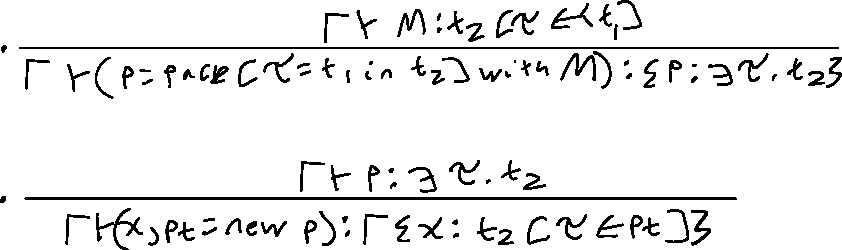
\includegraphics[width=\textwidth]{meta/cs349/ADT_Rules.pdf}{}
\end{center}
\end{figure}
\FloatBarrier
\textbf{
\item The pack[...] provides signatures of methods and the with ... provides implementations of methods
\item The ... = ... at the beginning of the pack provides a type for which the only value occupying is ``self''/``this'' for the use of the in ...
\item \underline{Note that even if the same ADT is constructed twice with the}\\
\underline{same internal representation, the returned ``objects'' will have}}\\
\underline{\textbf{different types} ($\tau_1$ $\neq$ $\tau_2$)} --- this is the only way in SLS of enforcing the fact that the ``methods'' of each instance are a collection of functions to be applied only to that instance
\end{itemize}
\clearpage
Example:\\
\verb|let point = [pack pt <: {x: num, y: num, active: bool} =|\\
\verb|{x:num, y:num, active: bool} in|\\
\verb|{create : num -> num -> pt, move : pt -> num -> num -> pt,|\\
\verb|switch : pt -> pt] with|\\
\verb|{create = \a:num. \b:num. {x=a, y=b, active=true},|\\
\verb|switch = \p.pt. if p@active=true then {x=p@x, y=p@x, false} else|\\
\verb|  {x=p@x, y=p@x, true}|\\
\verb|};|\\
\verb|p, T = new point;|\\
\verb|p1 = p@create 4 5;|\\
\verb|p2 = p@switch;|\\
Note, as we do not have mutability, every updating operation returns a new ``object'' (of the same ``self'' type). \textbf{The use of (bounded) sub-typing with the existential quantification is only necessary to provide ``getter''s}.
\subsection{Sub-typing relationships of bounded quantified types}
\FloatBarrier
\begin{figure}[h]
\begin{center}
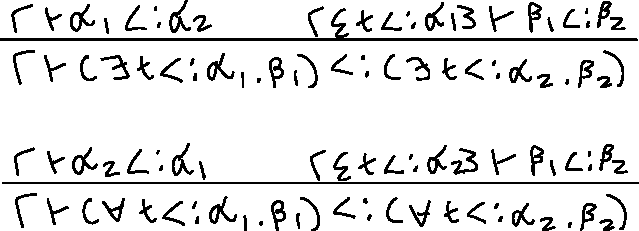
\includegraphics[width=0.67\textwidth]{meta/cs349/BoundedQuantificationRules.pdf}{}
\end{center}
\end{figure}
\FloatBarrier
That is that \textbf{existential quantification is co-variant in its type parameters whereas universal quantification is contra-variant in its type parameters}. It is intuitive that an ADT which exposes a superset of getters will be a safe substitution. The contra-variance is less intuitive a priori but consider the fact that all meaningful (ok yes, this is hand-wavy) universally quantified types are functions which take parameters of types of the type parameters and that functions are contravariant in their arguments.
\end{flushleft}
\end{document}